% ==========================================
% 第二篇 导入过场页
% ==========================================
\cleardoublepage
\thispagestyle{empty} % 让过场页干干净净，没有页眉页脚

\vspace*{6cm} % 整体垂直向下偏移，营造留白的高级感

\begin{center}
	% 篇章标题
	{\heiti\erhao 第二篇\quad 我们创造了什么} 
	\addcontentsline{toc}{part}{第二篇\quad 我们创造了什么}
	
	\vspace{2cm} % 标题与文案之间的间距
	
	% 灵魂文案
	{\songti\xiaosi \textit{“这不是卖一张更贵的卡，而是定义一个品类；\\ [0.5em] 这不是做一次交易，而是构建一个面向未来二十年的物理安全生态。”}}
\end{center}

\vfill
\cleardoublepage % 过场页结束，下一页正式开始第三章正文


% ==========================================
% 第三章
% ==========================================
\chapter{产品与技术方案}

\section{产品架构总览}

本方案针对通用门禁场景在量子计算时代面临的核心安全风险，构建了\textbf{“芯片-卡片-终端-平台”全链路抗量子安全架构}。依托团队在\textbf{武汉大学密码学与区块链实验室}的深厚技术积累，以自主研发的高性能后量子密码（PQC）算法库为核心底座，自上而下分为卡片层、读卡器层、后台层三个核心层级，实现端到端量子安全防护，同时完全兼容现有门禁系统，支持存量系统的平滑迁移。

本架构的核心设计原则包括：
\begin{enumerate}
	\item \textbf{全链路抗量子安全}：所有核心身份认证、密钥协商环节均采用NIST标准化的PQC算法，彻底抵御Shor算法对ECC/SM2的破解风险。
	\item \textbf{密码敏捷性设计}：底层算法栈支持热切换与动态升级，可快速适配未来标准与国密后量子算法，避免硬件替换成本。
	\item \textbf{全场景兼容适配}：向下兼容ISO 14443/15693、M1卡、国密CPU卡等现有生态，实现无感化后量子升级。
	\item \textbf{高性能低功耗优化}：针对门禁无源卡片、低功耗特性，对核心算法进行硬件与工程级深度优化，满足非接触式毫秒级响应。
\end{enumerate}

\begin{table}[htbp]
	\centering
	\caption{整体架构与核心技术能力}
	\renewcommand{\arraystretch}{1.3}
	\begin{tabular}{cp{4.5cm}p{4cm}p{5cm}}
		\toprule
		\textbf{层级} & \textbf{核心产品} & \textbf{核心能力} & \textbf{底层技术支撑} \\
		\midrule
		\textbf{卡片层} & PQC门禁卡 \newline (内置自主PQC安全SE芯片) & 后量子身份认证、双向密钥协商、凭证安全存储 & ML-KEM密钥封装、ML-DSA签名、国密算法、混合密钥推导 \\
		\textbf{读卡器层} & PQC门禁读卡器 \newline + PQC-SAM安全模块 & PQC协议解析处理、双向身份认证、OTA升级 & 嵌入式PQC算法优化、SAM硬件隔离、固件验签 \\
		\textbf{后台层} & 量子安全密钥管理平台 \newline (Quantum-Safe KMS) & 密钥全生命周期管理、密码敏捷性引擎、安全监控 & 分布式密钥存储、算法热切换、国密合规与等保适配 \\
		\bottomrule
	\end{tabular}
\end{table}

本架构的技术底座采用创新的\textbf{四层解耦合架构}设计，可实现跨芯片、跨终端的无缝适配：
\begin{itemize}
	\item \textbf{基础算子层}：提供有限域运算、矩阵向量乘加、大数运算等统一底层算力。
	\item \textbf{多项式运算层}：集成深度优化的NTT/INTT变换、多项式采样与规约算法。
	\item \textbf{哈希函数与采样层}：提供Keccak海绵结构、SHAKE可扩展输出及高斯/均匀采样。
	\item \textbf{算法实现与协议层}：拼装实现ML-KEM/ML-DSA等标准算法，并面向门禁场景提供APDU指令与认证协议集。
\end{itemize}

如下页图所示，通过高复用的底层算子设计，我们的代码体积明显减小，更好适配门禁卡此类嵌入式场景。
\begin{figure}
	\centering
	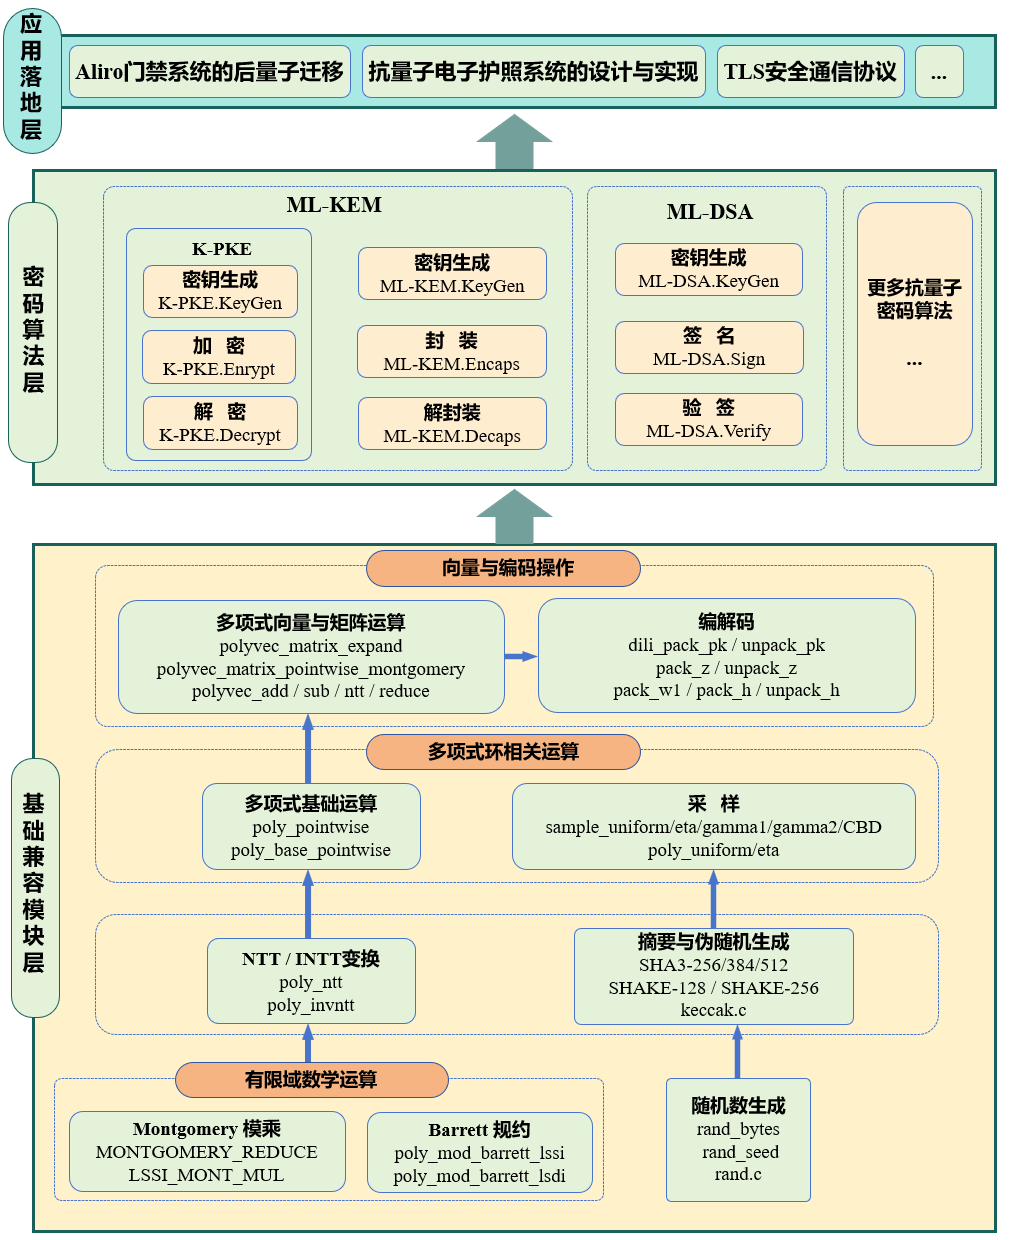
\includegraphics[width = \textwidth ]{figures/structures.png}
	
\end{figure}

\section{芯片层：PQC安全元件（SE）}

PQC安全元件是本方案的核心硬件信任根，专为门禁低功耗、高安全需求设计，是国内首款针对门禁场景优化的软硬协同抗量子安全芯片。\textbf{目前团队已与汇鼎科技等头部芯片厂商达成初步合作意向}，正推进PQC算法在物联网SE芯片上的流片与适配验证。

\subsection{芯片核心硬件架构}

采用“安全核+PQC协处理器+存储控制+通信接口”的四级架构：
\begin{enumerate}
	\item \textbf{32位安全主控核}：采用符合国密二级要求的RISC-V内核，内置硬件TRNG，支持内存隔离，密钥明文永不暴露到隔离区外。
	\item \textbf{专用PQC硬件协处理器}：针对格密码设计专用流水线，内置NTT加速单元与蒙哥马利模乘单元，运算速度比纯软件提升17倍以上。
	\item \textbf{国密算法硬件引擎}：内置SM1/SM4/SM7/SM2/SM3加速模块，与PQC引擎共享资源，实现双体系并行。
	\item \textbf{安全存储单元}：内置eFlash/ROM，支持防篡改、防物理攻击，密钥不可导出。
	\item \textbf{非接触式通信接口}：支持NFC无源模式（最高424kbps），针对PQC大尺寸密文优化通信帧结构，降低交互耗时。
\end{enumerate}

\subsection{内置PQC算法栈与底层数学实现}

\subsubsection{核心支持算法清单}

\begin{table}[htbp]
	\centering
	\caption{SE芯片内置核心支持算法}
	\renewcommand{\arraystretch}{1.2}
	\begin{tabular}{lllp{5.5cm}}
		\toprule
		\textbf{算法类别} & \textbf{算法名称} & \textbf{标准合规性} & \textbf{核心应用场景} \\
		\midrule
		抗量子密钥封装 & ML-KEM 512/768 & NIST FIPS 203 & 门禁双向密钥协商、会话密钥生成 \\
		抗量子数字签名 & ML-DSA 44/65 & NIST FIPS 204 & 门禁卡身份认证、固件签名验签 \\
		抗量子哈希签名 & SLH-DSA & NIST FIPS 205 & 根证书签名、长期身份凭证签名 \\
		国密对称算法 & SM1/SM4/SM7 & GM/T 0001-2012 & 门禁数据端到端加密、卡片存储加密 \\
		国密公钥算法 & SM2 & GM/T 0003-2012 & 兼容现有国密门禁、双算法混合认证 \\
		国密哈希算法 & SM3 & GM/T 0004-2012 & 数据摘要、挑战值生成、哈希绑定 \\
		\bottomrule
	\end{tabular}
\end{table}

\subsubsection{底层数学运算优化}

芯片内置算法库严格遵循格密码数学理论，针对无源低功耗场景做了深度定向优化：
\begin{enumerate}
	\item \textbf{多项式环运算}：基于商环 $\mathcal{R}_q=\mathbb{Z}_q[X]/(X^n+1)$ 构建核心运算。针对ML-KEM ($q=3329, n=256$) 和 ML-DSA ($q=8380417, n=256$)，采用负循环卷积实现多项式乘法，将复杂度从 $\mathcal{O}(n^2)$ 降至 $\mathcal{O}(n\log n)$。
	\item \textbf{数论变换（NTT）加速}：内置Cooley-Tukey正向NTT与GS逆向NTT硬件流水线。针对ML-KEM参数特性，优化了二次模乘的基乘运算，解决了512次本原单位根缺失带来的复杂度问题。
	\item \textbf{模约简算法优化}：集成Montgomery与Barrett双模约简。Montgomery用于NTT蝶形运算，引入基 $R=2^{32}$ 将模乘转化为移位与乘加；Barrett约简用于实现\textbf{常数时间执行}，抵御时序侧信道攻击。
	\item \textbf{采样算法实现}：内置CBD（中心二项分布）等专用采样，基于SHAKE进行伪随机数扩展，严格消除侧信道泄露风险。
	\item \textbf{紧凑编解码模块}：针对公钥和密文设计紧凑编码，序列化公钥长度压缩至 $32 + k \times 384$ 字节，大幅降低非接触式通信开销。
\end{enumerate}

\subsubsection{算法性能对标}

与业内主流开源PQC库（如PQ-magic）相比，本方案在门禁受限环境中实现了显著的性能跃升：

\begin{table}[htbp]
	\centering
	\caption{核心算法性能对标（基于相近主频MCU环境）}
	\renewcommand{\arraystretch}{1.2}
	\begin{tabular}{lccc}
		\toprule
		\textbf{算法/操作} & \textbf{本方案 (时钟周期)} & \textbf{业内开源库 (时钟周期)} & \textbf{性能提升} \\
		\midrule
		ML-DSA-44 密钥生成 & 233,121 & 586,151 & \textbf{+60.2\%} \\
		ML-DSA-44 签名验证 & 247,464 & 546,125 & \textbf{+54.7\%} \\
		ML-DSA-65 密钥生成 & 435,309 & 1,066,442 & \textbf{+59.2\%} \\
		ML-DSA-65 签名验证 & 488,229 & 925,238 & \textbf{+47.2\%} \\
		\bottomrule
	\end{tabular}
\end{table}

\subsection{安全防护与合规设计}
本方案具备\textbf{硬件级防侧信道攻击机制}（支持掩码防护、电磁屏蔽、时序混淆）、\textbf{硬件防火墙隔离机制}，设计符合《商用密码产品认证规则》，可支持国密二级与EAL5+安全认证。

\section{卡片层：后量子门禁卡}

\subsection{物理与通信规格}
完全符合 ISO 7816 ID-1 标准，支持定制封装。兼容 ISO 14443 A/B 和 ISO 15693 协议，无源模式读卡距离 $\ge$ 5cm，\textbf{单次完整认证流程耗时 $\le$ 300ms}，满足快通行需求。

\subsection{核心安全机制}

\textbf{1. 经典+PQC混合认证模式} \\
为平衡前瞻性与兼容性，采用“SM2/AES+ML-DSA/ML-KEM”\textbf{双轨并行认证}。两路认证独立执行、结果并行校验，单侧算法失效不影响整体安全边界。

\textbf{2. 混合密钥推导机制} \\
独立生成传统会话密钥 $K_1$ 与抗量子会话密钥 $K_2$，通过标准化HKDF函数进行绑定派生：
\[ K_{final} = \text{HKDF}(\text{SHA3-512}, K_1 \parallel K_2) \]
该机制彻底杜绝了单算法被攻破导致的会话密钥泄露风险。

\textbf{3. 防克隆与一次一密} \\
卡内密钥与SE芯片序列号\textbf{硬件绑定}，不可被克隆至其他芯片；每次刷卡通过双重随机挑战值（Challenge）派生全新密钥，确保刷卡数据\textbf{一次一密}，彻底杜绝嗅探与重放攻击。

\subsection{卡内APDU指令集实现}
卡片内置完整的扩展APDU指令集，不仅支持 `0x84` 获取传统挑战值、`0x82` 外部认证，更针对PQC协议增加了后量子专用指令族（如 `CLA=0x80`, `INS=0xB1` 获取PQC公钥，`0xB2` ML-KEM密钥封装等），完全兼容 ISO 7816-4 规范。

\section{读卡器层：PQC门禁读卡器}

读卡器内置 \textbf{PQC-SAM安全模块}，支持PQC协议终端侧处理及多协议向下兼容（M1卡/国密CPU卡）。

\subsection{核心功能与技术实现}

\begin{itemize}
	\item \textbf{多协议并行认证引擎}：自动识别卡片类型匹配协议。针对混合认证卡片，并行执行双链路认证而不增加额外耗时。
	\item \textbf{OTA安全固件升级}：采用 ML-DSA+SM2 \textbf{双算法固件验签}，A/B双分区防变砖设计，杜绝供应链攻击与恶意固件刷入。
	\item \textbf{抗量子认证协议 (PQ-Aliro)}：采用2-RTT两轮往返交互模式。第一阶段利用 ML-KEM 进行临时密钥交换；第二阶段使用 ML-DSA 进行双向签名认证与上下文哈希绑定。在不增加交互轮次的前提下完成强身份认证。
\end{itemize}

\subsection{嵌入式算法优化 (非公平优势体现)}
在MCU资源受限环境下，团队利用四层解耦合架构实现了极限优化：
\begin{enumerate}
	\item \textbf{深度代码复用}：ML-KEM与ML-DSA\textbf{完全复用底层的NTT模块}、多项式运算与哈希模块，大幅压缩固件体积，Flash占用减少超35KB。
	\item \textbf{流式哈希处理}：引入 Init-Update-Final 模式，无需将长报文一次性读入RAM，峰值内存占用降低60\%。
	\item \textbf{零拷贝数据处理}：算法直接操作通信缓冲区指针进行原地位解码，内存搬运延迟降低40\%。
\end{enumerate}

\section{后台层：量子安全密钥管理平台}

平台（Quantum-Safe KMS）采用微服务架构，分为接入层、服务层、数据层。为全系统提供统一的密码服务能力。

\begin{itemize}
	\item \textbf{密钥全生命周期管理}：依托硬件密码机生成真随机数，实现PQC与国密密钥的批量生成、安全分发、自动轮换与合规销毁。
	\item \textbf{密码敏捷性引擎 (Crypto-Agility)}：全算法采用插件化封装。支持算法版本、参数的\textbf{在线热切换}与灰度升级，无需更换底层硬件即可应对未来密码标准的演进。
	\item \textbf{智能安全监控}：基于规则引擎与机器学习识别异常刷卡（如高频、异地、防重放探测），自动触发设备锁定，并生成不可篡改的区块链审计日志。
\end{itemize}

\section{与现有最高端产品的全面对比}

本方案相较于当前业内最高端的高频门禁卡（MIFARE DESFire、国密SM2 CPU卡），在安全前瞻性与底层机制上实现了代际跨越：

\begin{table}[htbp]
	\centering
	\caption{门禁核心技术能力代际对比}
	\label{tab:comparison}
	\renewcommand{\arraystretch}{1.3}
	\small
	\begin{tabular}{p{2cm}p{3.5cm}p{3.5cm}p{5cm}}
		\toprule
		\textbf{能力维度} & \textbf{MIFARE DESFire} & \textbf{国密 CPU卡} & \textbf{本方案：后量子门禁卡} \\
		\midrule
		\textbf{公钥认证} & ECC-256 (\textbf{量子不安全}，可被Shor算法破解) & SM2 (\textbf{量子不安全}，可被Shor算法破解) & \textbf{ML-DSA} (NIST标准抗量子算法，量子安全) \\
		\textbf{密钥协商} & ECDH (\textbf{量子不安全}) & SM2 密钥协商 & \textbf{ML-KEM} (NIST抗量子密钥封装) \\
		\textbf{防克隆机制} & UID+AES 加密防护 & CPU芯片+国密算法 & \textbf{PQC+国密双重认证}，硬件根信任深度绑定 \\
		\textbf{合规前瞻性} & 不满足2030+抗量子要求 & 不满足2030+抗量子要求 & \textbf{符合NIST最新标准}，预留国密后量子演进接口 \\
		\textbf{密码敏捷性} & 固定算法栈，升级需换卡 & 固定算法栈，升级需换卡 & \textbf{底层算子解耦，算法可热更新} \\
		\textbf{侧信道防护} & 基础防护，无针对性设计 & 硬件级防护 & 硬件掩码+时序混淆+核心算法\textbf{常数时间执行} \\
		\textbf{协议交互} & 2-RTT单算法认证 & 2-RTT单算法认证 & \textbf{2-RTT双算法并行认证}，不增加额外耗时 \\
		\textbf{认证耗时} & ECC验签约 1.2ms & SM2验签约 1.5ms & \textbf{软硬协同优化 $\le$ 5ms}，满足门禁极速响应体验 \\
		\bottomrule
	\end{tabular}
\end{table}
